\documentclass[10pt]{Beamer}
\usepackage{fancybox}
\usepackage[most]{tcolorbox}
\usepackage{tikz}
\usepackage[utf8]{inputenc}
\usepackage{graphicx}
\usepackage[utf8]{inputenc}

\usetheme{Warsaw}

\title{Impactos da Creche na Primeira Infância: Efeitos Dependendo das Características da Família e do Grau de Exposição ao Centro de Cuidado}
\subtitle{Seminário de Econometria I}

\author{Lorenzo Costa \& Thallyta Marques}
\institute{Universidade Federal do Tocantins}
\date{\today}

\begin{document}
	
\frame{\titlepage}
\frame{\tableofcontents}

\section{Objetivo do Artigo}

\frame{
\frametitle{Objetivo do Artigo}

\begin{itemize}
	
\begin{block}

\item A

\end{block}

\vskip0,5cm

\begin{block}

\item B

\end{block}
	
\end{itemize}	

}

\section{Introdução}
\begin{frame}{A Motivação Para o Desenvolvimento do Trabalho}
\end{frame}

\section{As 5 Etapas do Modelo Econométrico}
	
	\subsection{Formulação do Problema}
	
\begin{frame}{A Formulação do Problema}
	

	
\end{frame}	


	\subsection{Bagagem Teórica}
	
\begin{frame}{O Modelo Teórico-Conceitual }
	
\end{frame}


	\subsection{Amostragem dos Dados}
	
\begin{frame}{Amostragem dos Dados}
	
\end{frame}


\begin{frame}{Variáveis do Modelo e Medição}
	
\end{frame}


	\subsection{Modelo Econométrico}

\begin{frame}{O Método e a Regressão Linear Múltipla}
	
\shadowbox{Structural Equation Modeling - SEM}	

\begin{figure}[h]
	\centering
	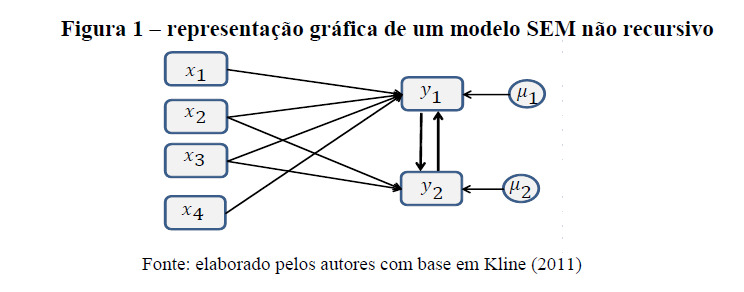
\includegraphics[width=0.8\textwidth]{SEM}
\end{figure}

\end{frame}

\begin{frame}{As Regressões}	

\begin{itemize}

\begin{block}
	
\item A equação básica do sistema de regressões é a seguinte: 

\end{block}

\end{itemize}

\begin{equation}
Y_{1i} = \alpha_1Y_{2i} + \beta_1creche_i + \beta_2familia_i + \beta_3criança_i + \beta4motivocrechei + \mu_i
\end{equation}

\begin{equation}
Y_{2i} = \alpha_1Y_{1i} + \beta_1creche_i + \beta_2familia_i + \beta_3criança_i + \beta_4motivocrechei + \mu_i
\end{equation}

\begin{tcolorbox}[drop fuzzy shadow=ShadowColor]
Em que $Y_{1i}$ representa o desempenho cognitivo ($cognitivo tvip$) e $Y_{2i}$ são os problemas externalizantes
\end{tcolorbox}

\end{frame}
	
\begin{frame}{As Regressões}

\begin{itemize}

\begin{block}

\item As equações que incluem as interações mencionadas e que permitirá verificar as diferenças dos efeitos da creche são:

\end{block}

\end{itemize}

\begin{equation}
Y_{1i} = \alpha_1Y_{2i} + \beta_1creche_i + \beta_2edumae_i + \beta_3creche.edumae_i + \beta_4familia_i \\ + \beta_5criança_i + \beta_6motivocreche_i + \mu_i
\end{equation}

\begin{equation}
Y_{1i} = \alpha_1Y_{2i} + \beta_1creche_i + \beta_2praticas_i + \beta_3creche.praticas_i + \beta_4familia_i \\ + \beta_5criança_i + \beta_6motivocreche_i + \mu_i
\end{equation}

\begin{equation}
Y_{1i} = \alpha_1Y_{2i} + \beta_1creche_i + \beta_2sens_i + \beta_3creche.sensib_i + \beta_4familia_i \\ + \beta_5criança_i + \beta_6motivocreche_i + \mu_i
\end{equation}

\end{frame}



	\subsection{Mensuração e Análise}
	
\begin{frame}{Resultado da regressão}
		
\end{frame}
	
\end{document}